\chapter{Controller Design}
	Previous sections of this report have discussed the necessary electronics as well the required mechanical structures for autonomous navigation inside a confined environment. This chapter describes the controller scheme necessary to enable such a platform to have stable flight in these areas.

	\section{Flight Control Strategy}
	Before a controller design can be accomplished, a detailed look into the high level control strategy must be done. \ref{IM_ControlStrategy} represents the controller scheme for \projectName. As shown, the controller is implemented as a sequence of embedded control loops, starting with way points being sent to the global position control, and ending with the most inner loop controlling the angular rates of the craft. Logically the controller can be split into 3 major components, which are discussed in the proceeding section. 
	
		\begin{figure}[H]
			\centering
			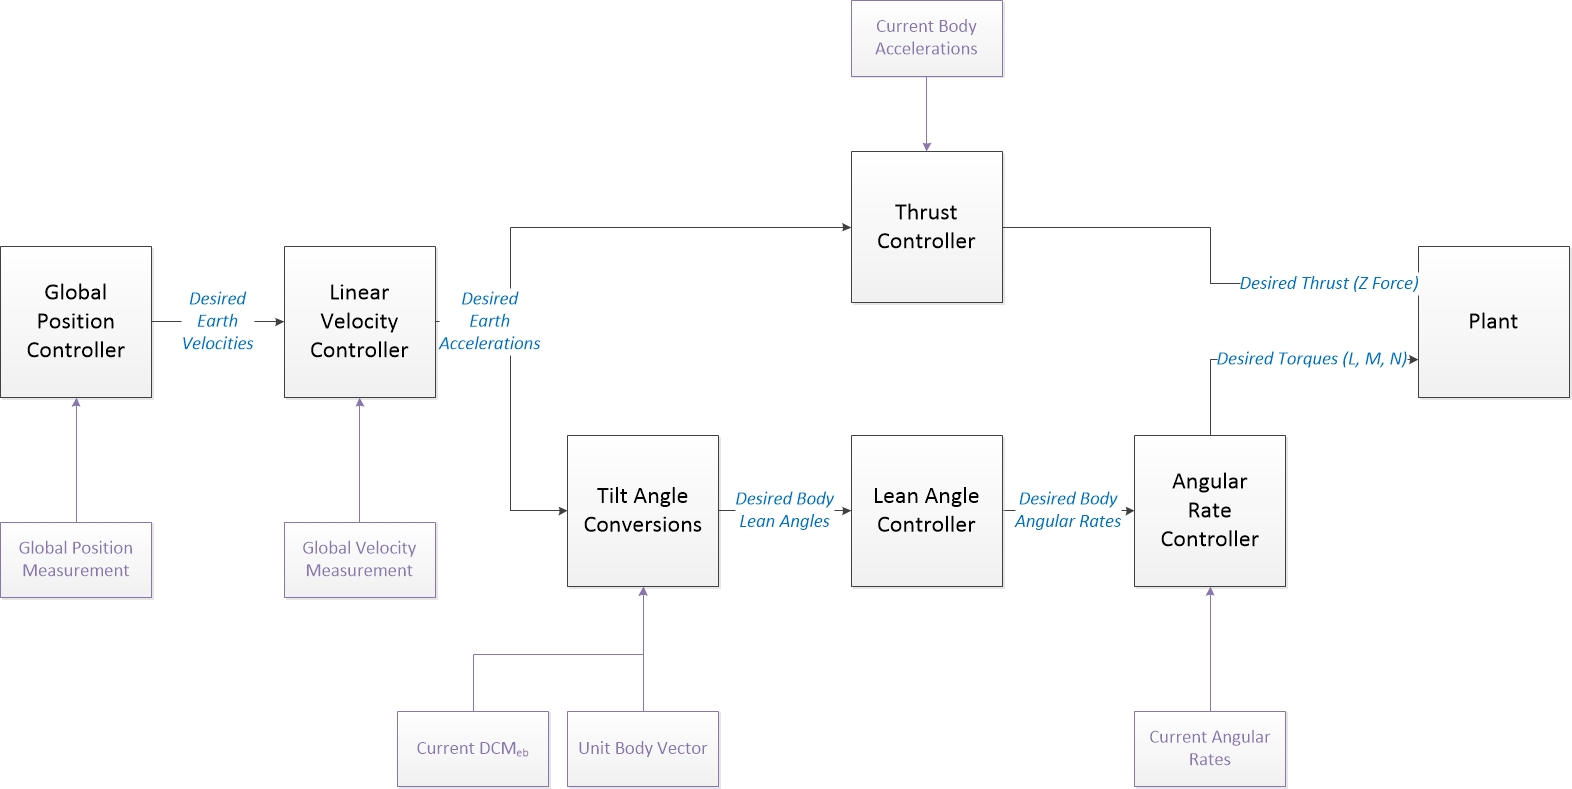
\includegraphics[height = 7.5cm]{../References/Diagrams/ControlDiagram.jpg}
			\caption{High Level Control Strategy}
			\label{IM_ControlStrategy}
		\end{figure}
		
		\subsection{Tracking Control}
		The onboard tracking control is seen as the software components that, given specific sensor data, can obtain autonomous stable flight. In this context autonomous implies the ability to follow given GPS locations. As shown in \ref{IM_ControlStrategy}, the tracking controller consisted of four main blocks. The  most inner loop is the angular rate controller, this block outputs desired moments and takes in angular rates as set points from the lean angle controller. The lean angle controller is given set points from the linear velocity controller, the conversions required are discussed in the tilt angle conversions section. The linear velocity controller has it's setpoints calculated by the global position controller. 
		Both the linear velocity controller and the global position tracking system, work in the North, East, Down frame. Whereas the inner angular controllers, work in the body frame. The thrust controller, along with the Tilt angle conversions are responsible for combining the two frames.
		
		\subsection{Near Wall Effect Control}
		As discussed in Section \ref{SSSECT_NearGroundEffect In Section}, close proximity to a wall or large surface can produce a disturbance on any rotorcraft. In \cite{NearWall}, a disturbance observer was the proposed method for controlling the effects of being close to a wall. in Section \ref{SectionDisturbanceObserver}, a generic disturbance based controller was discussed. This chapter looks closer at the implementation of that control and the effect it has on the tracking system.
		As discussed below, the near wall disturbance has been modelled as a thrust loss based on proximity of a specified rotor to a wall. This is observed by... and controlled with... (feeding back estimation values)
		\todo[inline]{Not Complete}
		
		\subsection{Assumptions and Limitations}
		In order to accurately model the craft, certain assumptions and limitations must be made. These quantification of these limitations are listed in \ref{TAB_UnitsLimits}. The forces and moments limits are set by the physical hardware, where as the limitations for angles and rates are derived from the high level flight strategy. 
		Due to the application in a confined space, the linear velocities will be kept low at all times. This limitation produces two effects on the system. Firstly, it limits the maximum lean angles of the craft and secondly it limits the nominal thrust used by the craft during translational movements. The lower nominal thrust gives the drone more headroom to handle disturbances effectively. The maximum thrust of the drone is dictated by the chosen motor, rotor pair. This is under the assumption that the ESCs chosen, can produce the maximum performance out of each motor. 
		The lean angle limit can intuitively be set low due too the desired slow translations. Due to the disturbance rejection often requiring quick responses in rate changes, the desired angular rate limit is set high.
		To calculate the largest possible moments the arm length of the drone must be taken into consideration. Since it is desired to never completely shut off one motor, each rotor will always produce some thrust, also limiting the maximum moment.
		\todo{Add in assumption about motor mixer providing maximum thrust and moment through an actuator? Probably not...}
		
		\begin{table}[!]
			\centering
			\begin{tabular}{l | c | c | c |}
				Parameter & Unit & Limit\\
				\hline\hline
				Thrust					& N 	& 50\\
				Moments					& Nm 	& 2\\
				Angular Rate 	   		& Rad/s & 1\\
				Lean Angle	    		& Rad 	& 0.35\\ %20 degrees
				Linear Velocity 	  	& m/s 	& 1\\
				Global Position  		& m 	& NA\\
			\end{tabular}
			\label{TAB_UnitsLimits}
			\caption{Controlled Parameters Units and Limits}
		\end{table}
		\todo{Finalise table values}
			
	\section{System Identification}
	In order to correctly model the system, a thorough system identification needs to be completed. This entails real world measurements of the chosen platform. The methods and results from these experiments are covered in this section.
	
		\subsection{Mass and Inertia}
		Using a calibrated scale the mass of the rotorcraft measured at 3.352Kg. To calculate moments of inertia, the Bifilar Pendulum method was used. The method is thoroughly described in literature and involves tying the drone from the ceiling allowing it rotate around one axis. Since it is desired to measure the inertias along three axes, three separate test set ups were required. Images of the test set up for a single axis is shown in \ref{IM_BifilarPendulum}. 
		
		\begin{figure}[H]
			\centering
			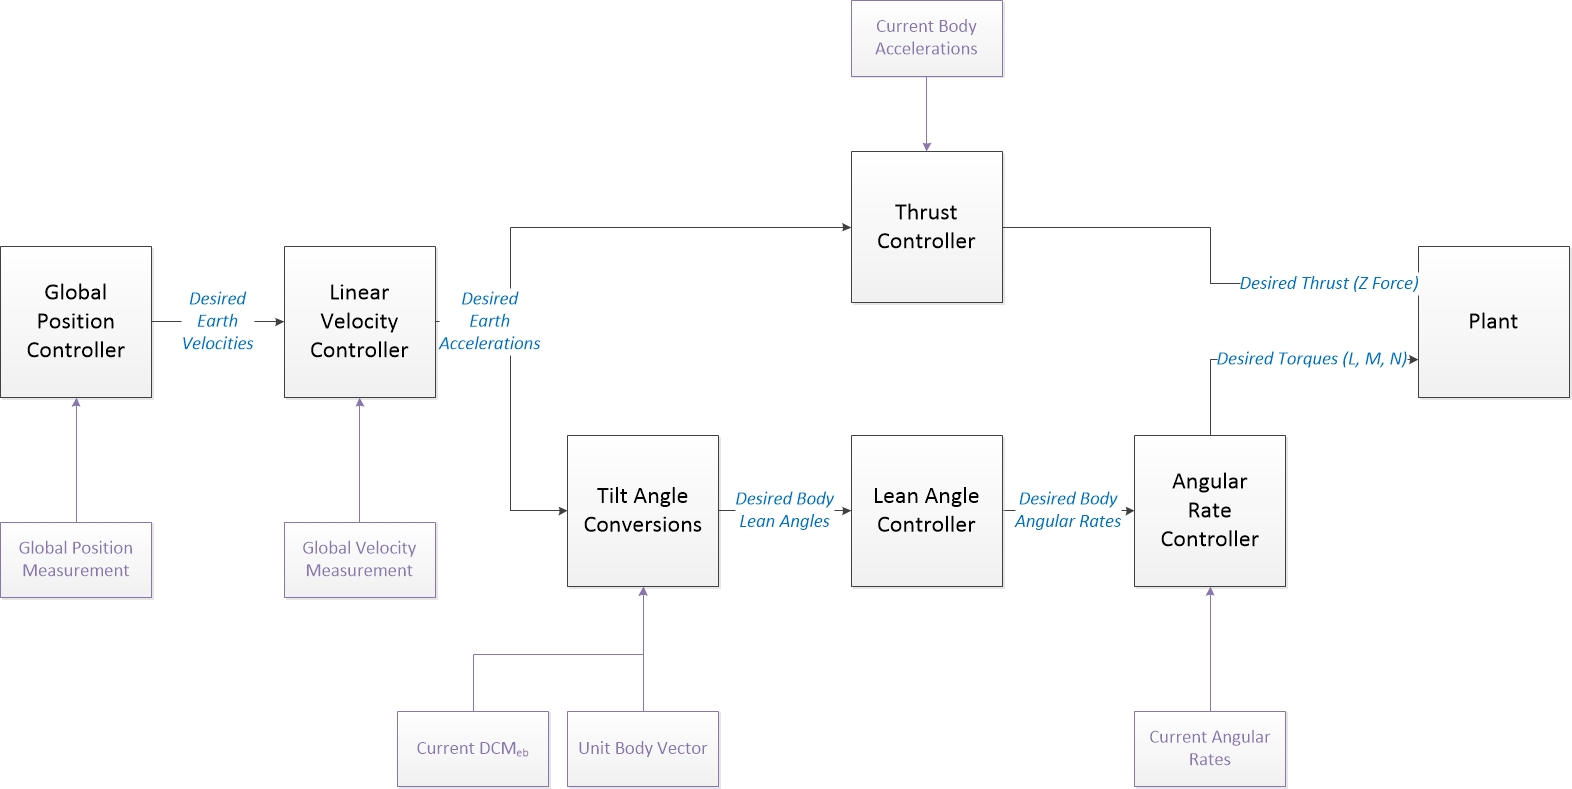
\includegraphics[height = 7.5cm]{../References/Diagrams/ControlDiagram.jpg}
			\caption{Bifilar Pendulum for Measurement}
			\label{IM_BifilarPendulum}
		\end{figure}
		
		Each axis was measured 10 times and the values were averaged out to obtain the final values represented in Table \ref{TAB_MomentOfInertia}. To give a representation of measurement variance, the standard deviation is provided along side.
				
		\begin{table}[!]
			\centering
			\begin{tabular}{l | c | c | c |}
				Parameter & Averaged Measured Value & Standard Deviation\\
				\hline\hline
				$I_{xx}$ & 0.025027578 & 0.001063842\\
				$I_{yy}$ & 0.169260024 & 0.000142928\\
				$I_{zz}$ & 0.170196714 & 0.000527406\\
			\end{tabular}
			\label{TAB_MomentOfInertia}
			\caption{Measured Moments of Inertia}
		\end{table}
		
		\subsection{Thrust and Moment Profiles}
		In order to correctly valid the thrust characteristics of the drone, each motor rotor pair needed to be evaluated. Each pair was marked and coupled to a load cell. The ESCs were configured to send varying PWMs to the motors. The commands sent to the ESCs and the measured thrust values are plotted together in Figure \ref{IM_ThrustProfiles}.
		
		\begin{figure}[H]
			\centering
			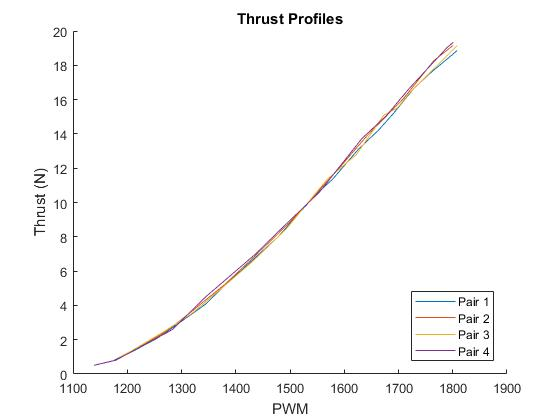
\includegraphics[height = 7.5cm]{../Design/Mechanical/ThrustProfiles/thrustprofiles.jpg}
			\caption{Bifilar Pendulum for Measurement}
			\label{IM_ThrustProfiles}
		\end{figure}
		
		\begin{table}[!]
			\centering
			\begin{tabular}{l | c | c | c |}
				Pair & Max Thrust & Min Thrust\\
				\hline\hline
				$1$ & 18.8558 & 0.7852\\
				$2$ & 19.1489 & 1.1889\\
				$3$ & 19.1434 & 0.9511\\
				$4$ & 19.3369 & 0.5087\\
			\end{tabular}
			\label{TAB_ThrustProfiles}
			\caption{Measured Moments of Inertia}
		\end{table}
		
		
		\subsection{Instrumentation}
		The dynamic flight model has been evaluated in Section \ref{SSECT_DynamicFLightModel}
			\subsubsection{Kalman Filter}
		
		\subsection{Disturbances}
			\subsubsection{Wind}
			\subsubsection{Drag}
			\subsubsection{Near Wall Effect}
	
	\section{Angular Rate Controller}
		\subsection{Roll}
		\subsection{Pitch}
		\subsection{Yaw}	

	\section{Lean Angle Controller}
		\subsection{Roll}
		\subsection{Pitch}
		\subsection{Yaw}			
	
	\section{Linear Velocity Control}
	
	\section{Tilt Angle Conversions}
	
	\section{Thrust Controller}
	
	\section{Global Position Tracking Control}
	
	\section{Disturbance Based Observer}
	